\documentclass[12pt,a4paper]{article}
\usepackage{composites2019}
\usepackage{booktabs}

\begin{document}
\thispagestyle{empty}

\vspace*{-3.4cm}
\begin{table}[!h]
\begin{tabular}{r}
\hspace*{5.5cm} \scriptsize \textsf{7th ECCOMAS Thematic Conference on the Mechanical Response of Composites} \\
\hspace*{5.5cm} \scriptsize \textsf{ COMPOSITES 2019} \\
\hspace*{5.5cm} \tiny \textsf{A. Turon, P. Maimí \& M. Fagerström (Editors)}
\end{tabular}
\end{table}

\begin{center}
\title{ESTIMATING THE AVERAGE SIZE OF FIBER/MATRIX INTERFACE CRACKS IN UD AND CROSS-PLY LAMINATES}
\end{center}
\begin{center}
\textbf{\underline{Luca Di Stasio}$^{1,2,*}$, Janis Varna$^{1}$, Zoubir Ayadi$^{2}$} \\ [7pt]
\small{$^1$~Lule\aa\ University of Technology, University Campus, SE-97187 Lule\aa, Sweden}  \\  [2pt]  
\small{$^2$~Universit\'e de Lorraine, EEIGM, IJL, 6 Rue Bastien Lepage, F-54010 Nancy, France}  \\  [2pt]
\small{$^*$~\texttt{luca.di.stasio@ltu.se}} \\
\end{center}


\paragraph{Keywords:} Fiber Reinforced Polymer (FRP), Debonding, Linear Elastic Fracture Mechanics (LEFM).

\paragraph{Summary:} \textit{This document provides information and instructions for preparing the (optional) full-length paper for the COMPOSITES 2019 Conference (September 18-20, 2019 in Girona, Spain).}

\section{INTRODUCTION}

The Conference publication will consist of a pen drive containing papers of the contributions received and a printed Book of Abstracts containing a one page version of the accepted abstracts. The authors must submit a full-length paper (max. 12 pages) using the same format of this template. Submission of a full-length paper is not mandatory but authors are strongly encouraged to send it before June 27, 2019.

The deadline date for early registration date is April 30, 2019. Presenting authors must register by June 13, 2019. Papers with authors not registered by this date will be removed from the final program.
Registration closes on September 5, 2019. Further information can be found at the conference website: \texttt{www.composites2019.udg.edu}

\section{RVE MODELS AND FE DISCRETIZATION}

In this contribution, we analyze debond initiation and propagation in Representative Volume Elements (RVEs) of Uni-Directional (UD) composites and $\left[0_{m\cdot k\cdot2L}^{\circ},90_{k\cdot2L}^{\circ},0_{m\cdot k\cdot2L}^{\circ}\right]$ laminates. Given a global reference frame with axis $x$, $y$ and $z$, both types of composites are modeled as plates lying in the $x-y$ plane, with the through-the-thickness direction thus aligned with the $z$ axis. The UD composite $0^{\circ}$ direction is parallel to the $y$ axis, while the cross-ply $0^{\circ}$ direction is parallel to the $x$ axis. Both composites are loaded in tension along the $x$ axis, which thus corresponds to: transverse loading of the UD specimen; axial loading of the cross-ply specimen. In both composites, damage is present only in the form of fiber/matrix interface cracks, or debonds. In cross-plies, debonds are assumed to be present only in the central ${90^{\circ}}$. Given that: first, in the presence of a load in the $x$-direction, the $y$-strain due to Poisson's effect is very small; second, debond size is assumed to be considerably larger in the fiber than in the arc direction~\cite{Zhang1997}; we can consider $2D$ models under plane strain conditions defined in the $x-z$ plane. UD composites and $90^{\circ}$ plies are characterized by a regular microstructure following a square-packing configuration of fibers, built through the repetition of a one-fiber unit cell along the horizontal and the vertical direction. This unit cell is a square with the center occupied by one fiber of radius $R_{f}=1\ \mu m$ and the rest of the element constituted by matrix. The size of the one-fiber unit cell is $2L\times 2L$, such that:

\begin{equation}\label{eq:LVf}
L=\frac{R_{f}}{2}\sqrt{\frac{\pi}{V_{f}}},
\end{equation}

where $V_{f}$ is the fiber volume fraction, here assumed to be $60\%$. It is worth to specify at this point that the choice $R_{f}=1\ \mu m$ is arbitrary and stems from the fact that the linear elastic solution, as the one considered in this article, is proportional to the geometrical dimensions of the model. Simplicity is thus the main reason for this choice. Also, $V_{f}$ is always the same in the one-fiber unit cell and the entire RVE, i.e. no fiber clustering is analyzed in this work. In the case of cross-ply laminates, the $0^{\circ}$ layer is homogenized with properties evaluated according to the Concentric Cylinders Assembly with Self-Consistent Shear (CCA-SCS) model~\cite{Hashin1983,Christensen1979}. A glass fiber-epoxy system is considered for both UDs and cross-ply laminates. Material properties are reported in Table~\ref{tab:phaseprop}.

\begin{table}[!htbp]
 \centering
 \caption{Summary of mechanical properties of fiber, matrix and UD layer.}%$E$ stands for Young's modulus, $\mu$ for shear modulus and $\nu$ for Poisson's ratio. Indexes $L$ and $T$ stand respectively for \emph{longitudinal} and \emph{transverse}.}
 \begin{tabular}{ccccccc}
\textbf{Material} & \textbf{$V_{f}\left[\%\right]$}\  & \textbf{$E_{L}\left[GPa\right]$}\ & \textbf{$E_{T}\left[GPa\right]$}\  & \textbf{$G_{LT}\left[GPa\right]$} &\textbf{$\nu_{LT}\left[-\right]$} & \textbf{$\nu_{TT}\left[-\right]$} \\
\midrule
Glass fiber &-   & 70.0 & 70.0  & 29.2 & 0.2  & 0.2\\
Epoxy    &-& 3.5 & 3.5   & 1.25 &  0.4& 0.4\\
UD&60.0&43.442&13.714& 4.315& 0.273&0.465\\
\end{tabular}
\label{tab:phaseprop}
\end{table}

The use of coupling conditions allows the study of a Repeating Unit Cells (RUC) of reduced size with respect to the corresponding RVE, which translates in a gain in terms of computational time and memory usage during the evaluation of Finite Element (FE) solution. The RVEs studied in this article are reported in Figure~\ref{fig:rves} with the corresponding RUC highlighted by dashed line (in blue in the online color version) and with symmetry and coupling conditions represented by rollers (
\includegraphics[scale=0.5]{roller.pdf}). Details about the central one-fiber unit cell are shown in Figure~\ref{fig:ruc}. Notice that the analysis, in terms of stresses and Energy Release Rate (ERR), is conducted on this central one-fiber unit cell, both in the case of an undamaged and of a partially debonded fiber.\\
Nomenclature and main features of the RVEs studied are described in the following.

\begin{description}
\item [$\mathbf{n\times k-free}$, Figure~\ref{fig:rves-a}: ]UD composite with thickness $t_{0^{\circ}}=k\cdot2L$, where $k$ is the number of fiber ``rows'' in the vertical (through-the-thickness) direction and $2L$ the side length of the one-fiber unit cell as defined in Equation~\ref{eq:LVf}. Debonds appear only in the central fiber ``row'' every $n-1$ fully bonded fibers on alternating sides of the partially debonded fiber, where $n$ is the number of fiber present in the RUC along the horizontal direction.
\item [$\mathbf{n\times k-coupling}$, Figure~\ref{fig:rves-b}: ]UD composite with infinite thickness. Debonds appear every $k-1$ fully bonded fibers along the vertical direction in a fiber ``column'', fiber ``columns'' containing debonds appear every $n-1$ ``columns'' of fully bonded fibers. Debonds are placed on the same side of the partially debonded fiber inside the same fiber ``column'', while they appear on alternating sides between one fiber ``column'' with damage to the next. The RUC has thus $n$ fibers in the horizontal and $k$ fibers in the vertical direction. Conditions of coupling of the vertical displacement are applied on the top side.
\item [$\mathbf{n\times k-asymm}$, Figure~\ref{fig:rves-c}: ]UD composite with infinite thickness. Debonds appear every $k-1$ fully bonded fibers along the vertical direction in a fiber ``column'', fiber ``columns'' containing debonds appear every $n-1$ ``columns'' of fully bonded fibers. Debonds are placed on opposite sides of the partially debonded fiber inside the same fiber ``column'' and they appear on alternating sides between one fiber ``column'' with damage to the next. The RUC has thus $n$ fibers in the horizontal and $k$ fibers in the vertical direction. The following set of conditions is applied to the upper boundary:

\begin{equation}\label{eq:asymm}
\begin{aligned}
u_{z}\left(x,kL\right)-u_{z}\left(0,kL\right)&=-\left(u_{z}\left(-x,kL\right)-u_{z}\left(0,kL\right)\right)\\
u_{x}\left(x,kL\right)&=-u_{x}\left(-x,kL\right)
\end{aligned}
\end{equation}

which represent conditions of anti-symmetric coupling~\cite{DiStasio2019b}.

\item [$\mathbf{n\times k-m\times t_{90^{\circ}}}$, Figure~\ref{fig:rves-d}: ]Cross-ply laminate with $90^{\circ}$ layer thickness $t_{90^{\circ}}=k\cdot2L$ and $0^{\circ}$ layer thickness $t_{0^{\circ}}=m\cdot t_{90^{\circ}}$. $k$ is the number of fiber ``rows'' in the vertical (through-the-thickness) direction of the $90^{\circ}$ layer and $2L$ the side length of the one-fiber unit cell as defined in Equation~\ref{eq:LVf}. Debonds are present only in the central fiber ``row'' of the $90^{\circ}$ layer every $n-1$ fully bonded fibers on alternating sides of the partially debonded fiber, where $n$ is the number of fiber present in the RUC along the horizontal direction.
\end{description}

\begin{figure}[!h]
\centering
    \subfigure[$n\times k-free$]{\label{fig:rves-a}\raisebox{0.085\textheight}{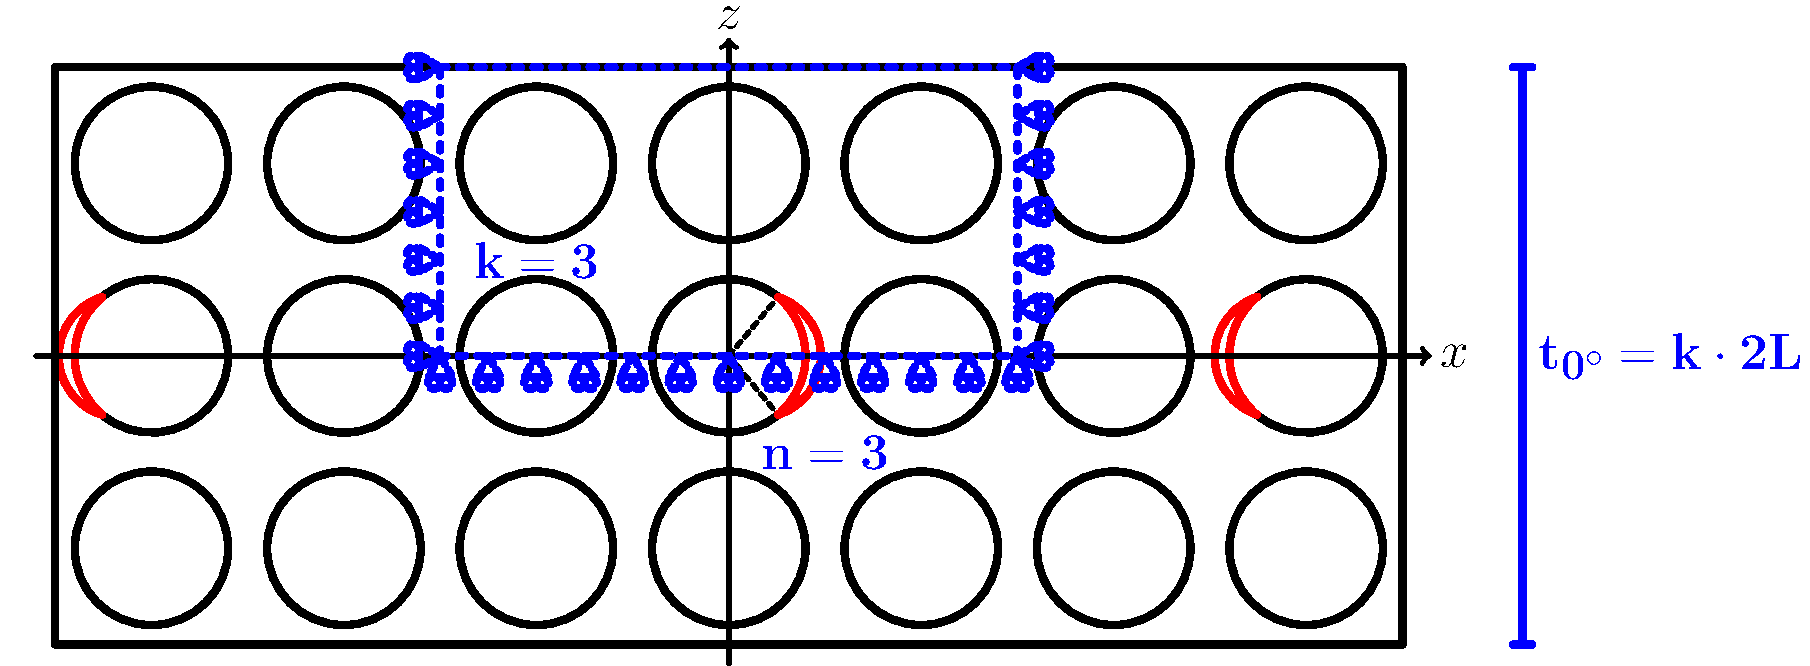
\includegraphics[width=0.485\textwidth]{thickPlyUD.pdf}}}\quad 
    \subfigure[$n\times k-coupling$]{\label{fig:rves-b}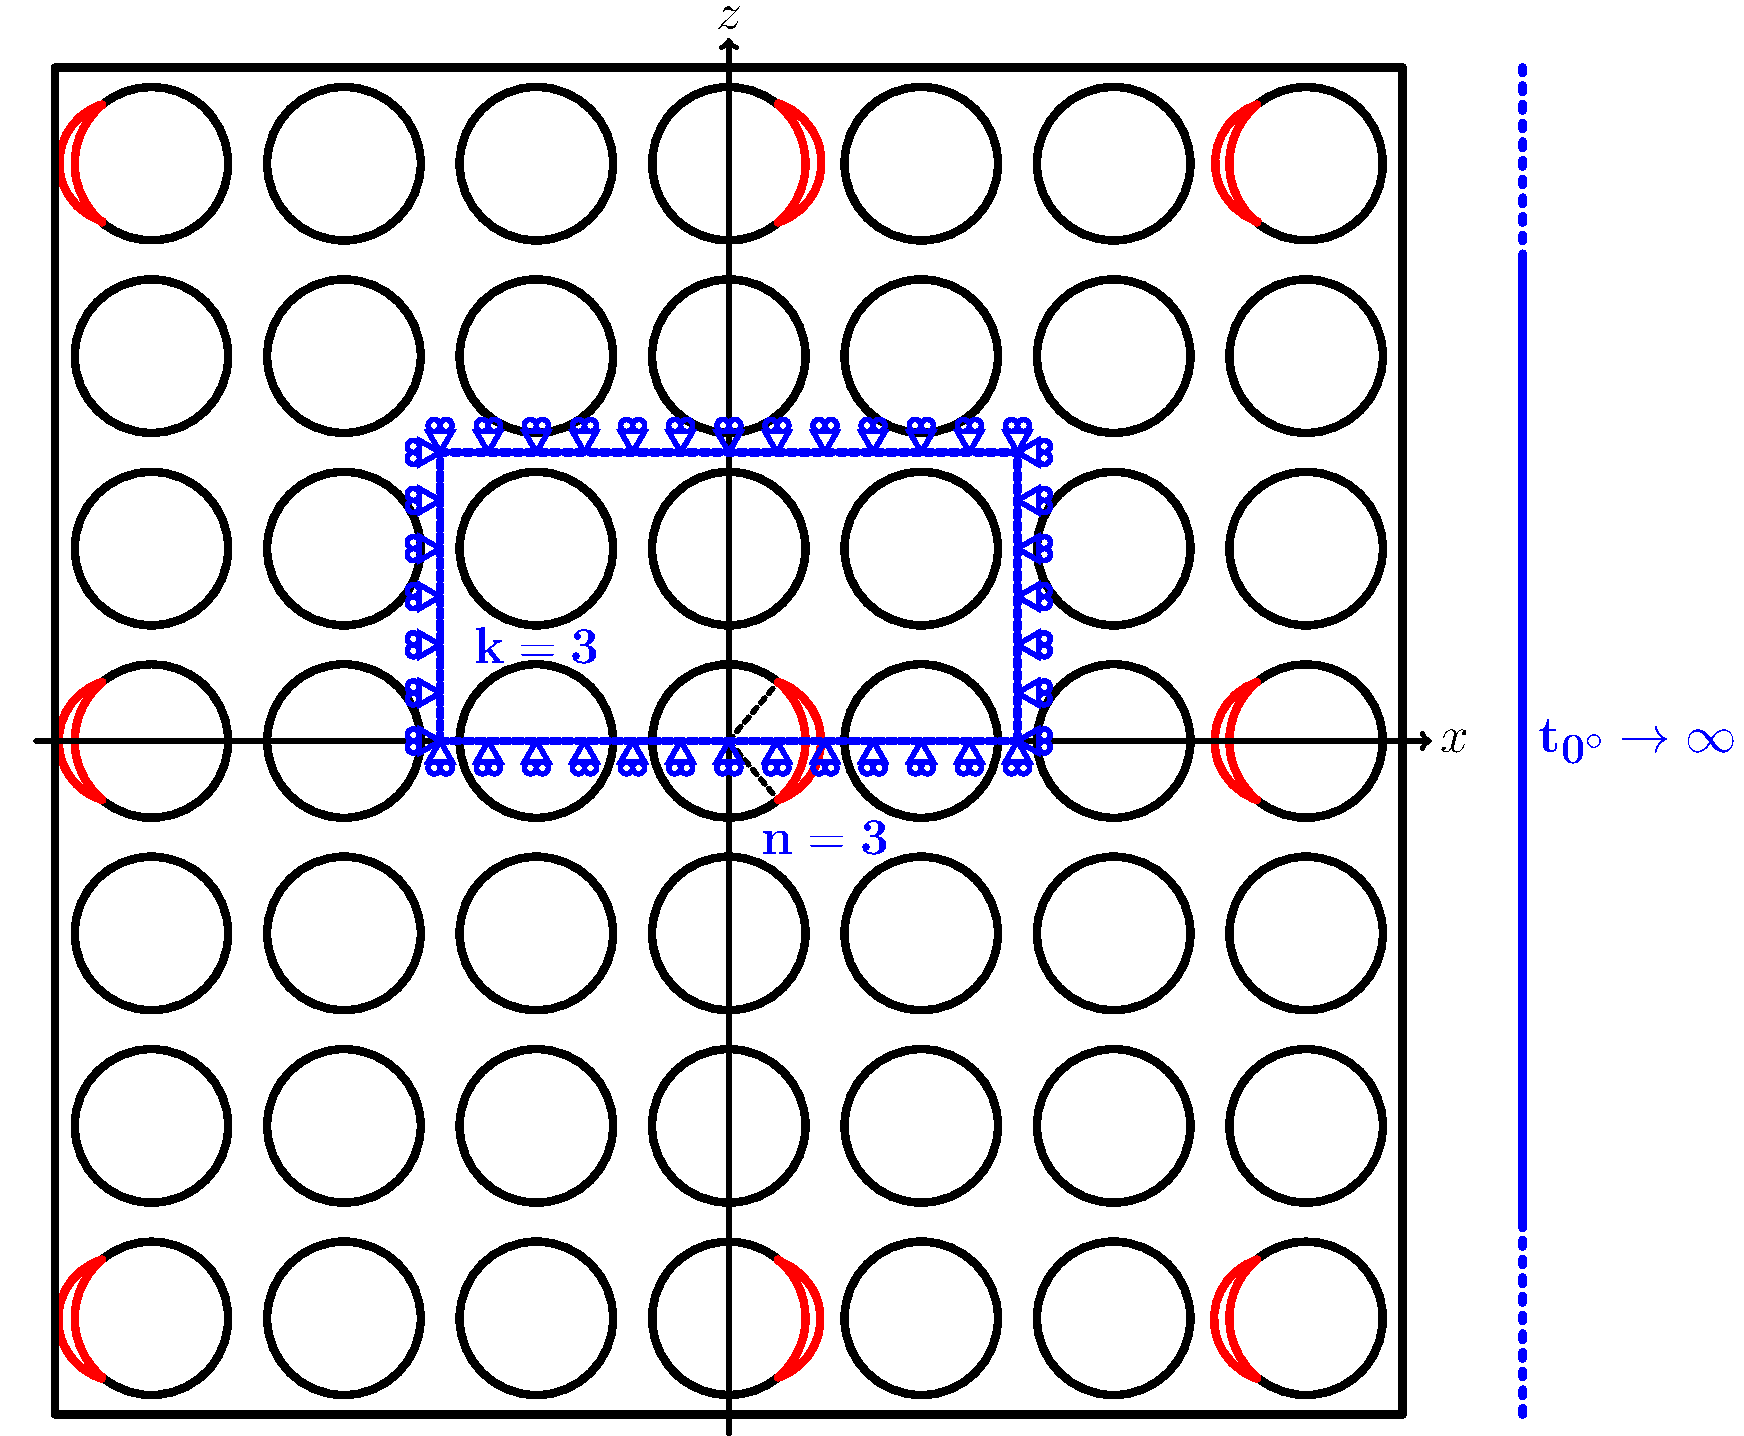
\includegraphics[width=0.485\textwidth]{coupling.pdf}}\\
    \subfigure[$n\times k-asymm$]{\label{fig:rves-c}\raisebox{0.03\textheight}{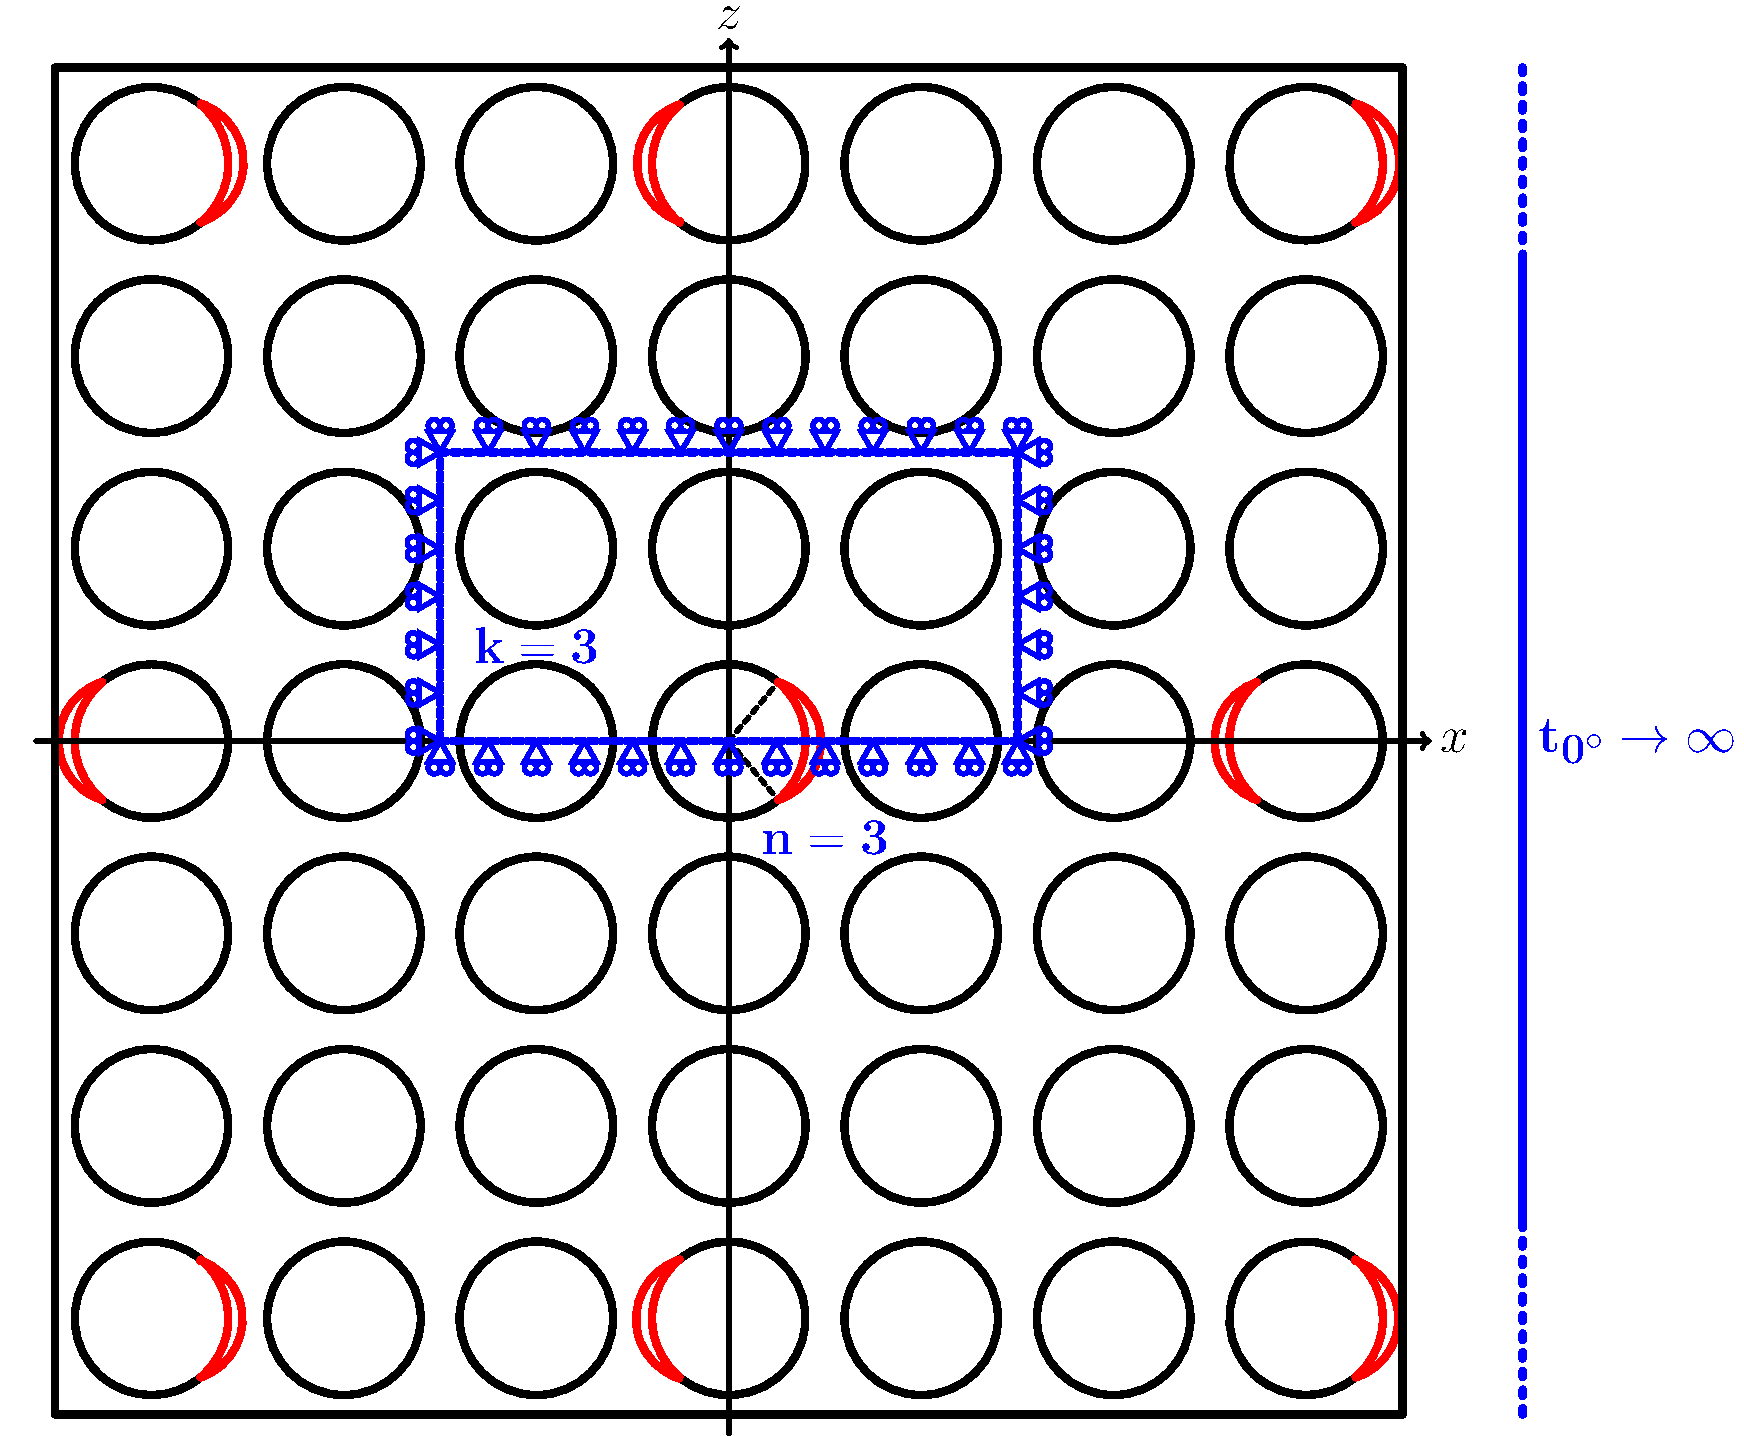
\includegraphics[width=0.485\textwidth]{asymm.pdf}}}\quad
    \subfigure[$n\times k-m\times t_{90^{\circ}}$]{\label{fig:rves-d}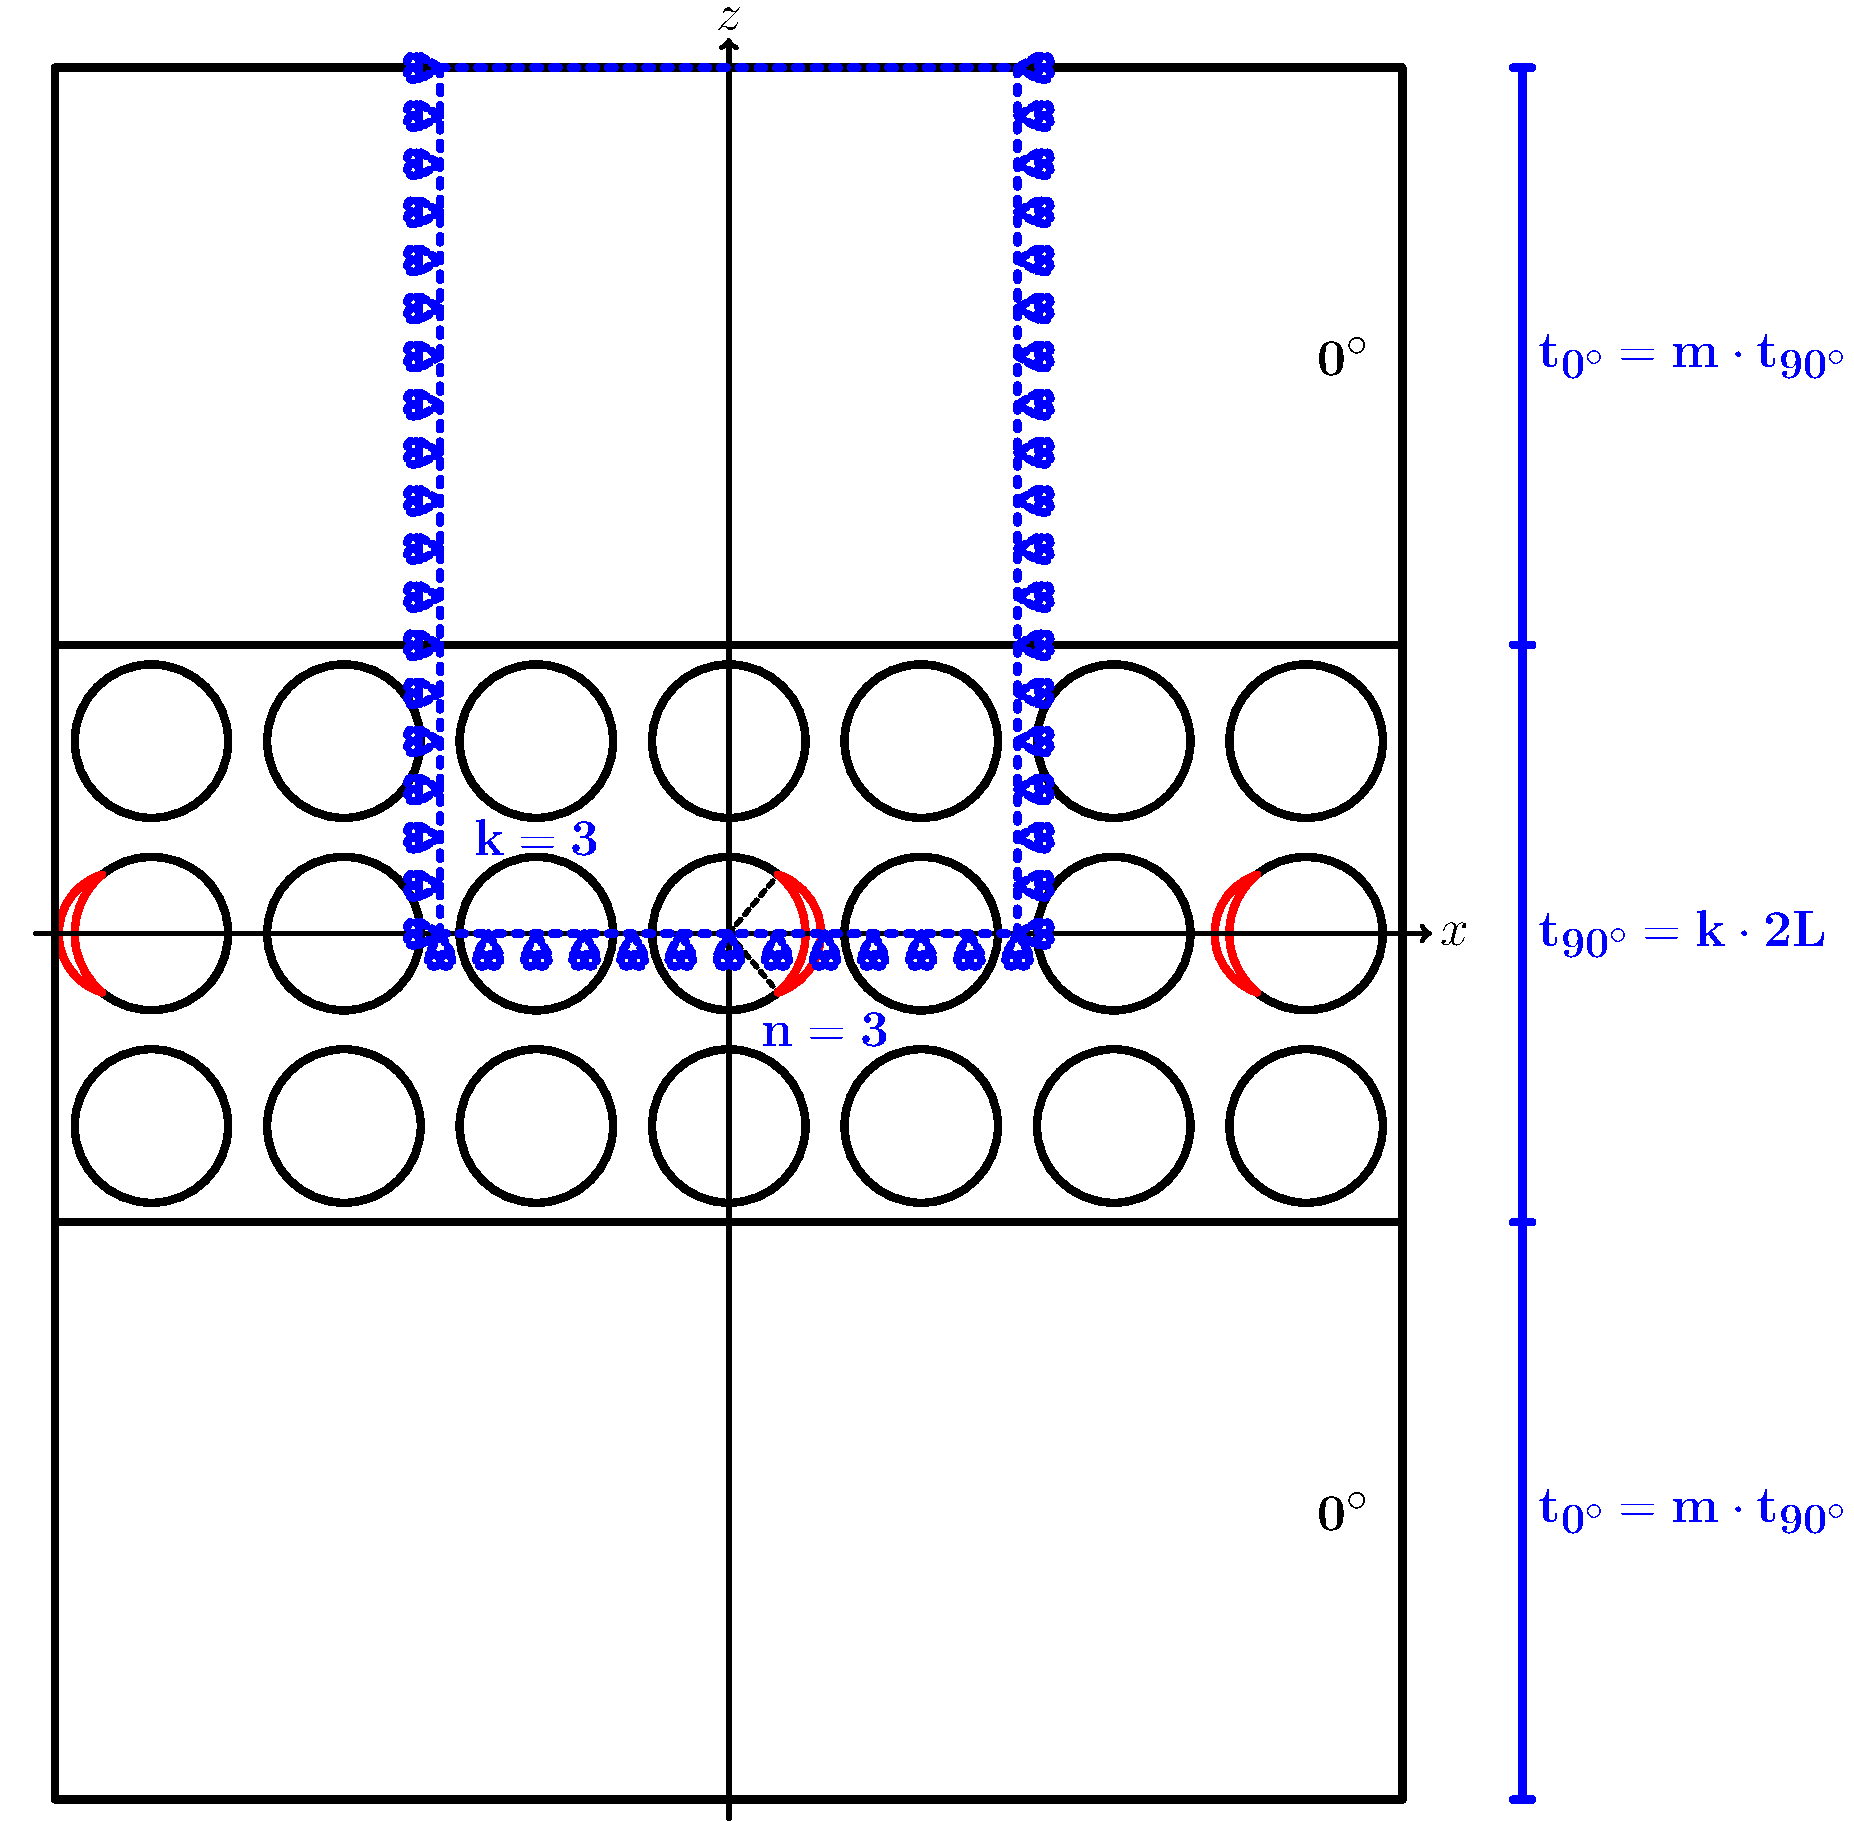
\includegraphics[width=0.485\textwidth]{ThickPlyCP.pdf}}
\caption{Composite RVEs and corresponding RUCs analyzed.}\label{fig:rves}
\end{figure}

Every RUC is symmetric with respect to the horizontal ($x$) direction, thus only half of it is modeled in the FE solution through the use of symmetry boundary conditions on the bottom side. Conditions of coupling of the horizontal displacement are applied on the left and right side, to model the repetition of the RUC along the horizontal direction. A tensile load is applied on the right and left side in the form of displacement $\bar{u}_{x}=\bar{\varepsilon}_{x}nL$ with $\bar{\varepsilon}_{x}=1\%$. The debond has a size of $2\Delta\theta$ (see Figure~\ref{fig:ruc}), with $\Delta\theta\geq0$ ($\Delta\theta=0$ is the case of no damage at all). For large debonds ($\Delta\theta\geq 60^{\circ}-80^{\circ}$), a region called \emph{contact zone}, of size $\Delta\Phi$ to be determined by the solution itself, appears at the crack tip. Correct resolution of this behavior requires the imposition of conditions of non-interpenetration of the crack faces. Crack faces contact is assumed to be frictionless.

\begin{figure}[!h]
\centering
        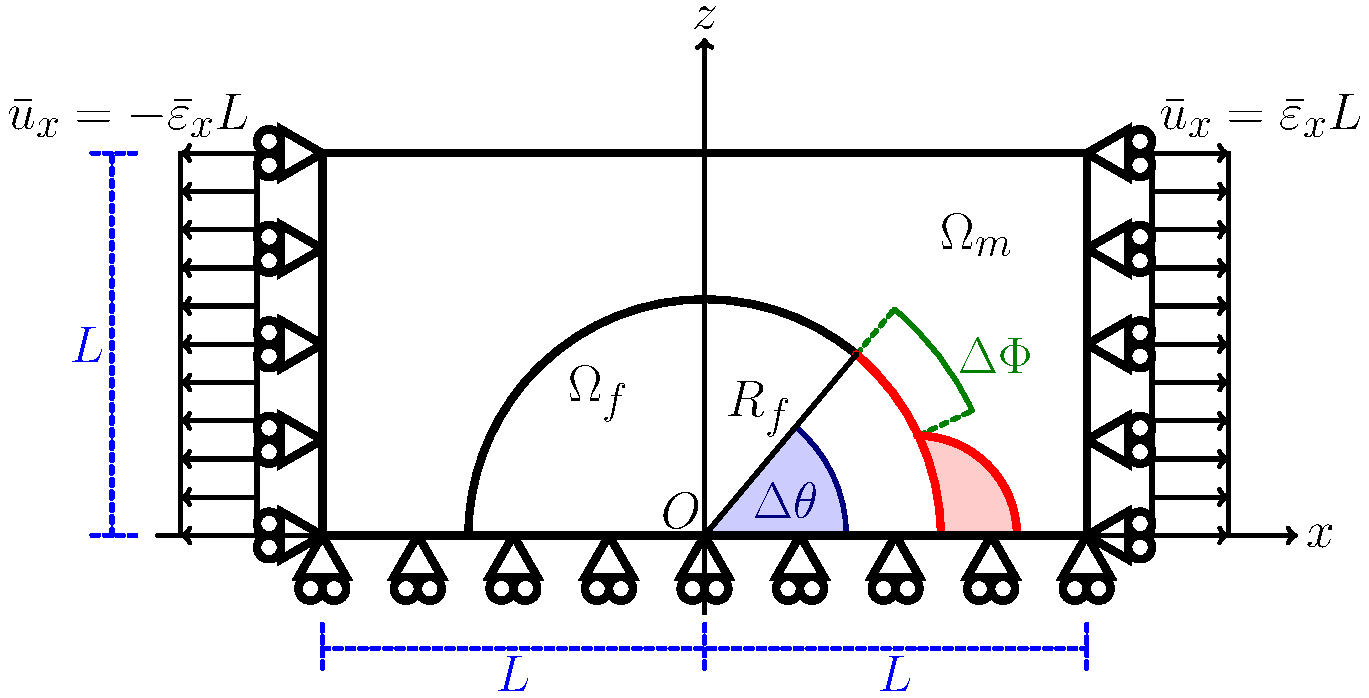
\includegraphics[height=0.25\textheight]{RUC.pdf}
\caption{One-fiber unit cell and main parameters characterizing the debonding process.}\label{fig:ruc}
\end{figure}

The FE solution is evaluated using Abaqus~\cite{abq12} using second order, 2D, plane strain triangular (CPE6) and rectangular (CPE8) elements. To correctly resolve the singularity at the crack tip, a regular mesh of only rectangular elements is used with almost unitary aspect ratio and angular size $\delta=0.05^{\circ}$. The crack faces are represented as element-based surfaces with frictionless small-sliding contact pair interaction.

\begin{figure}[!h]
\centering
        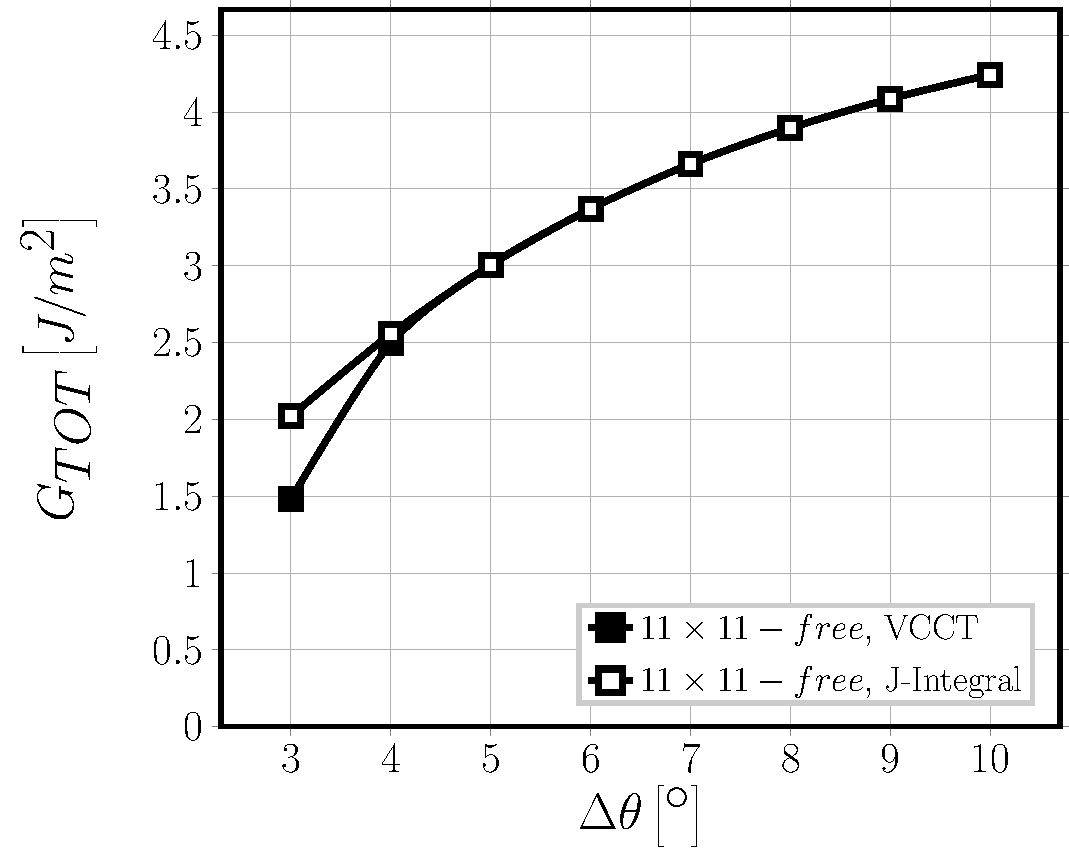
\includegraphics[height=0.3\textheight]{vf60-G-methodsaccuracy.pdf}
\caption{Comparison of total ERR of $11\times11-free$ evaluated respectively with VCCT and J-integral.}\label{fig:errerror}
\end{figure}

Mode I ERR is underestimated with the Virtual Crack Closure Technique (VCCT)~\cite{Krueger2004} for very small debonds (see Figure~\ref{fig:errerror}), due to the high $\frac{\delta}{\Delta\theta}$ ratio. Thus, for $\Delta\theta<10^{\circ}$, $G_{TOT}$ is evaluated using the J-integral~\cite{Rice1968}, $G_{II}$ with the VCCT and $G_{I}$ as $G_{TOT}=G_{I}+G_{II}$; for $\Delta\theta\geq10^{\circ}$ only the VCCT is used. Validation of the model is performed with respect to BEM results of~\cite{Paris2007,Sandino2016}; the order of accuracy of the results (differences $\leq5\%$ are not significant) is discussed in~\cite{DiStasio2019}.

\section{STRESS-BASED ANALYSIS OF DEBOND INITIATION}

The distribution of stresses at the fiber/matrix interface is analyzed in models $1\times k-free$ and $1\times k-1\cdot t_{90^{\circ}}$ with $k=1,3,11,201$ and $\Delta\theta=0^{\circ}$, i.e. the undamaged case. Some selected stress components are analyzed, based on their relevance in previous studies on debond initiation and growth: the radial $\sigma_{rr}$ and shear $\tau_{r\psi}$ stress~\cite{Mantic2009}, the Local Hydrostatic Stress (LHS, following the notation of~\cite{Carraro2016}) $\sigma_{LHS}$~\cite{Asp1996a,Asp1996b}, the local von Mises stress $\sigma_{vM}$~\cite{Canal2012}, the Local Maximum Principal Stress (LMPS, following the notation of~\cite{Carraro2016}) $\sigma_{LMPS}$~\cite{Carraro2014}. In plane strain conditions there exists an out-of-plane axial component of the stress ($\sigma_{yy}$ in our notation): in order to study the importance of this out-of-plane component (tri-axial stress state, see~\cite{Asp1995}), $\sigma_{LHS}$, $\sigma_{vM}$ and $\sigma_{LMPS}$ are evaluated both neglecting (index $2D$) and considering (index $3D$)  $\sigma_{yy}$.

\begin{figure}[!h]
\centering
    \subfigure[$\sigma_{rr}$]{\label{fig:stress-a}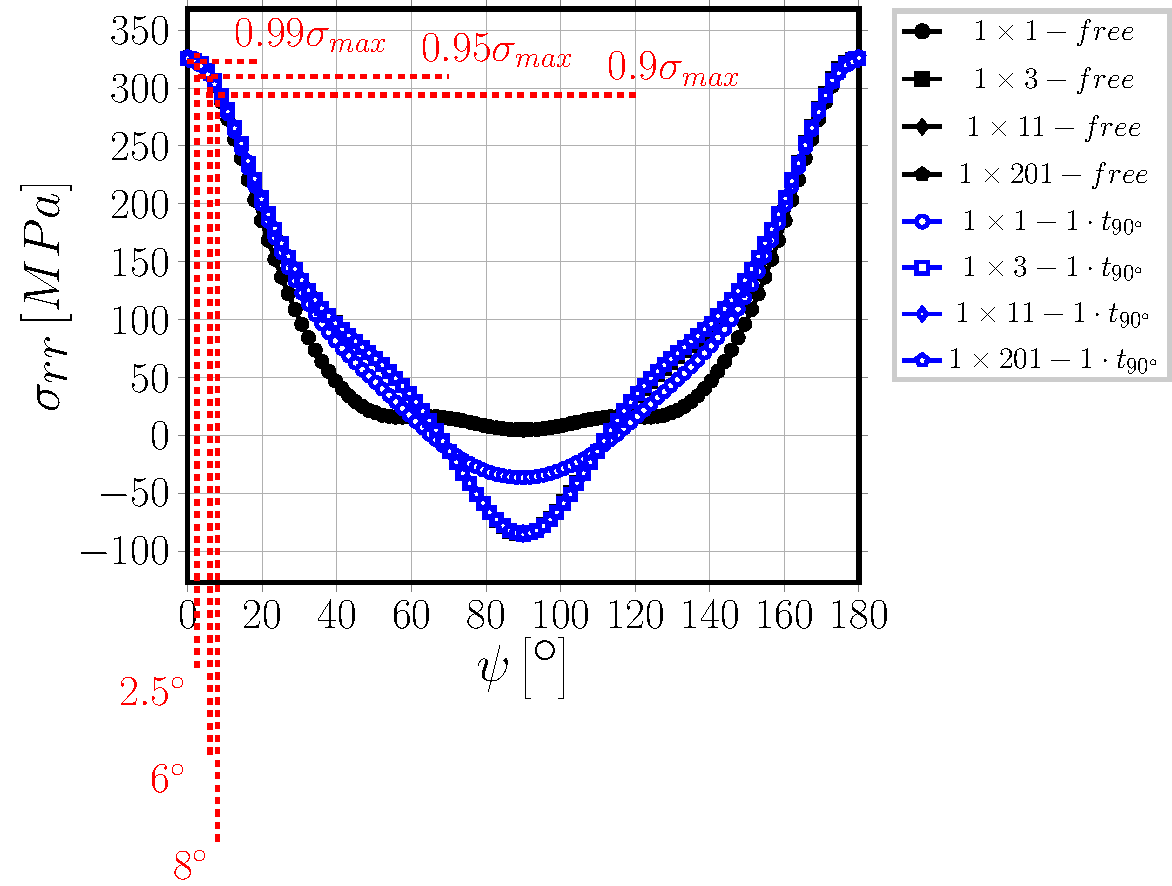
\includegraphics[height=0.22\textheight]{vf60-nodamage-sigmar.pdf}}\  
    \subfigure[$\tau_{r\psi}$]{\label{fig:stress-b}\raisebox{0.04\textheight}{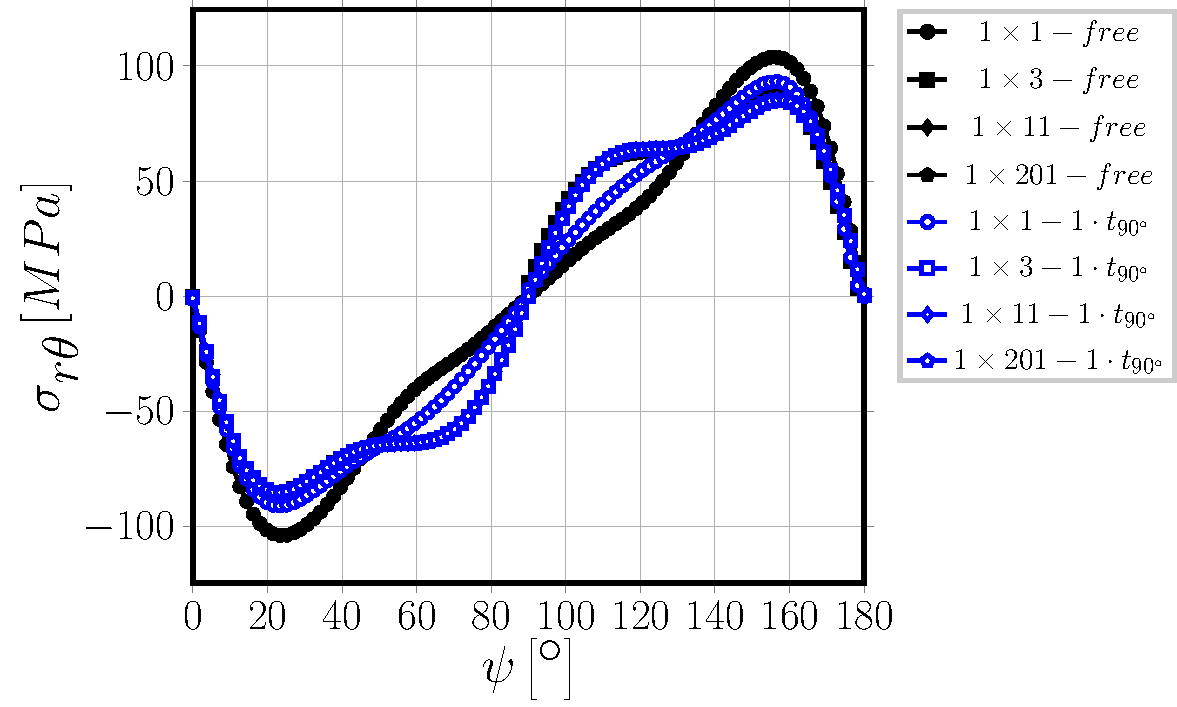
\includegraphics[height=0.18\textheight]{vf60-nodamage-taurt.pdf}}}\\
    \subfigure[$\sigma_{LHS,2D}$]{\label{fig:stress-c}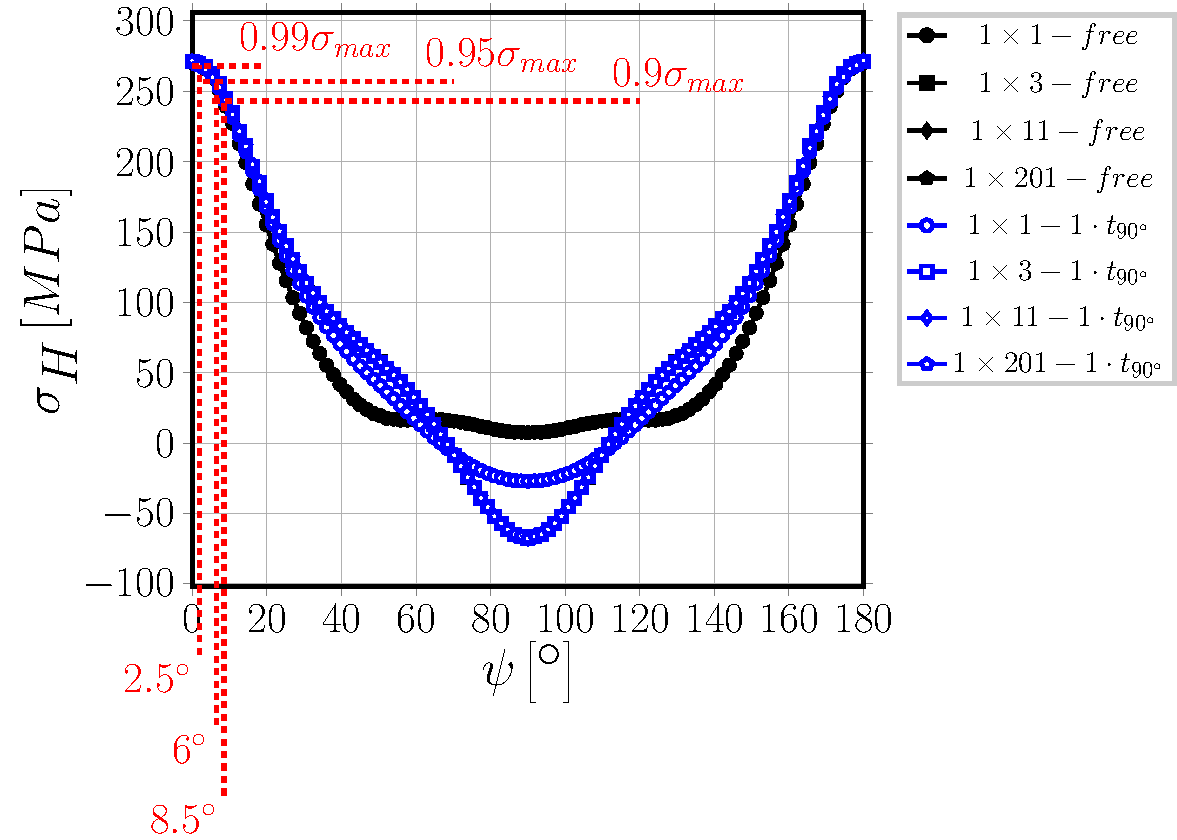
\includegraphics[height=0.22\textheight]{vf60-nodamage-p2D.pdf}}\ 
    \subfigure[$\sigma_{LHS,3D}$]{\label{fig:stress-d}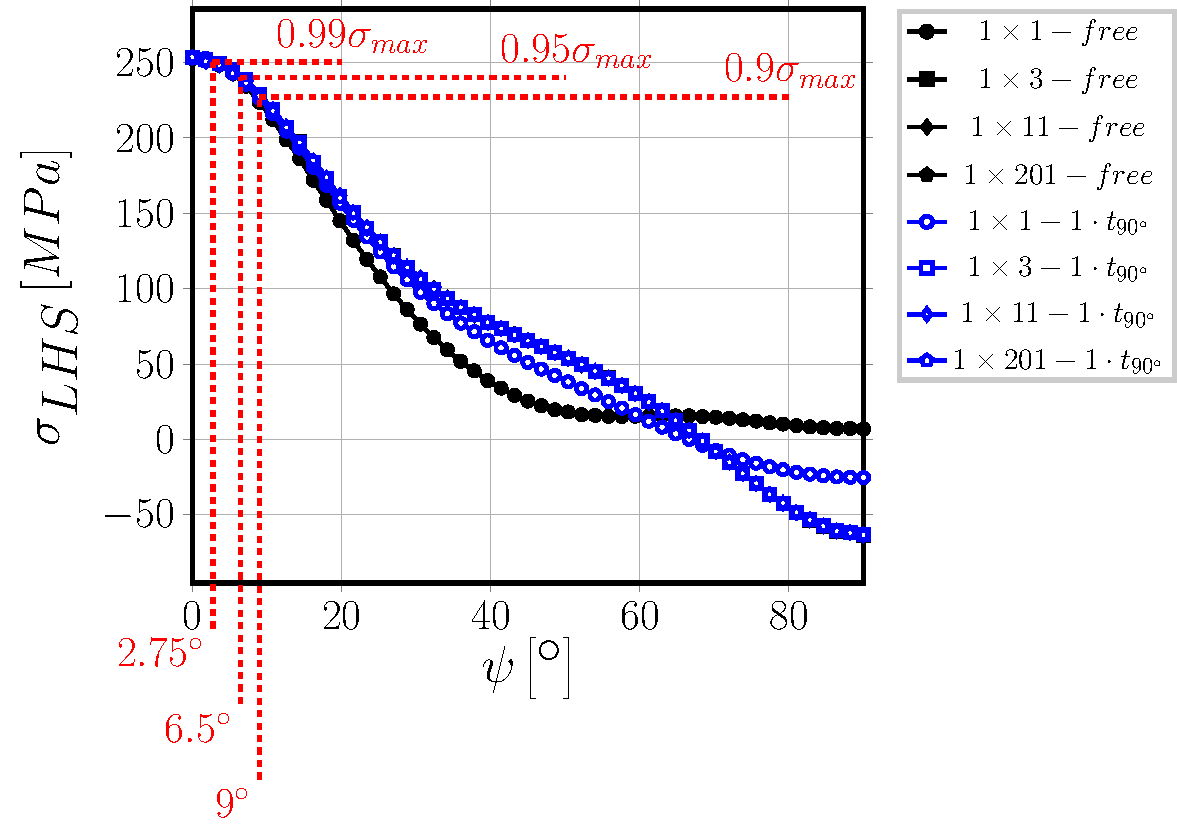
\includegraphics[height=0.22\textheight]{vf60-nodamage-p3D.pdf}}
    \subfigure[$\sigma_{vM,2D}$]{\label{fig:stress-e}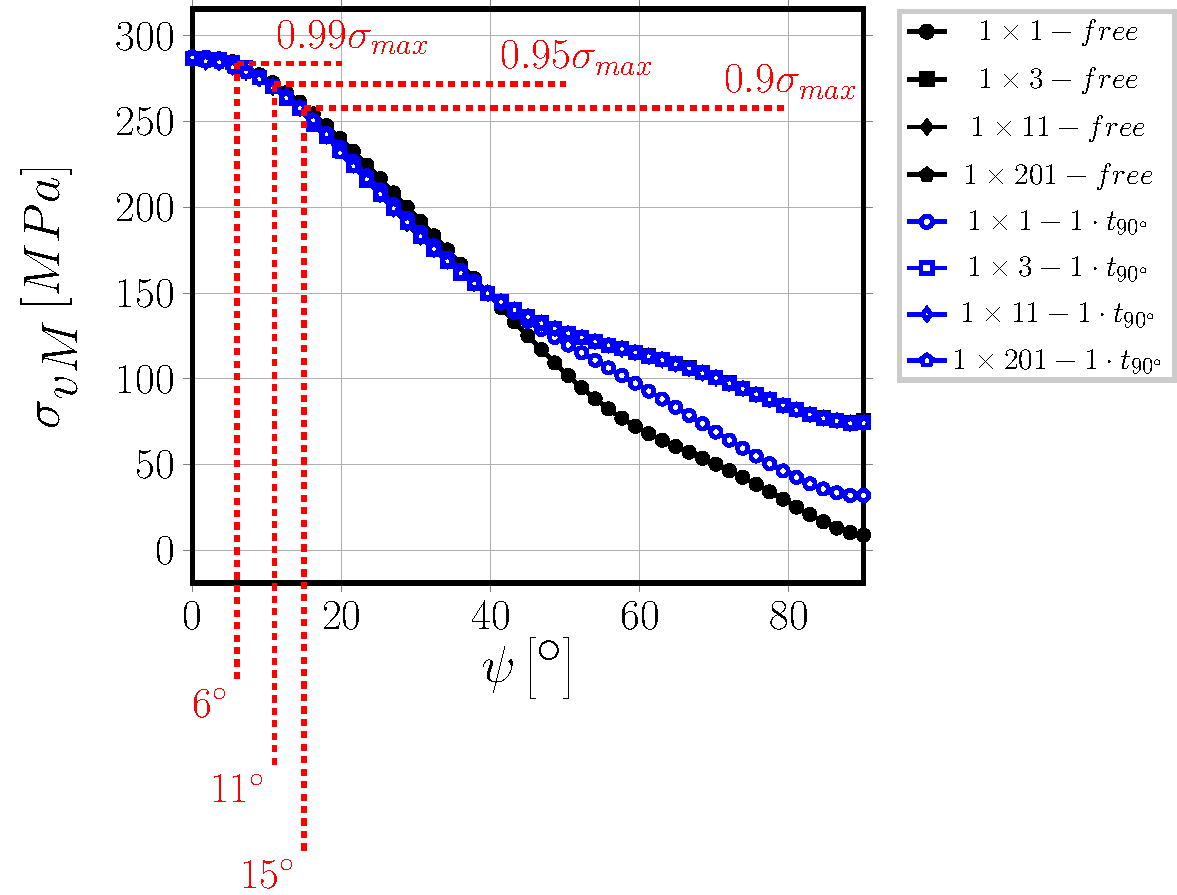
\includegraphics[height=0.22\textheight]{vf60-nodamage-vM2D.pdf}}\ 
    \subfigure[$\sigma_{vM,3D}$]{\label{fig:stress-f}\raisebox{0.04\textheight}{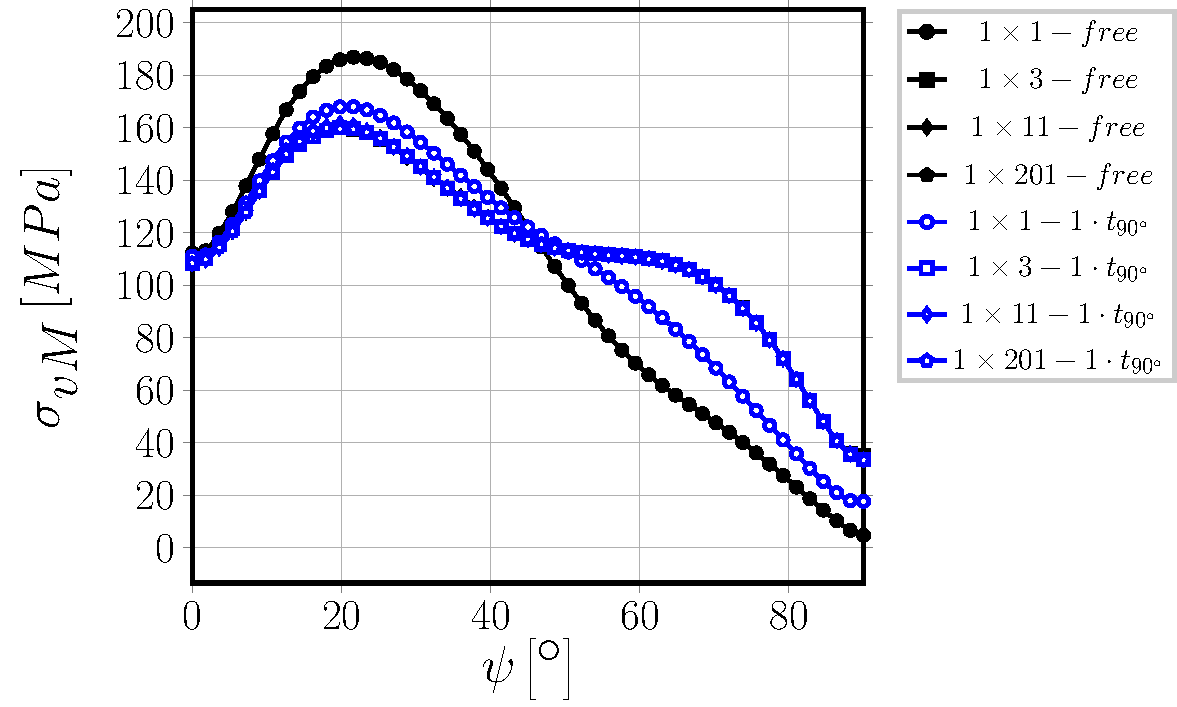
\includegraphics[height=0.18\textheight]{vf60-nodamage-vM3D.pdf}}}
    \subfigure[$\sigma_{LMPS,2D}$]{\label{fig:stress-e}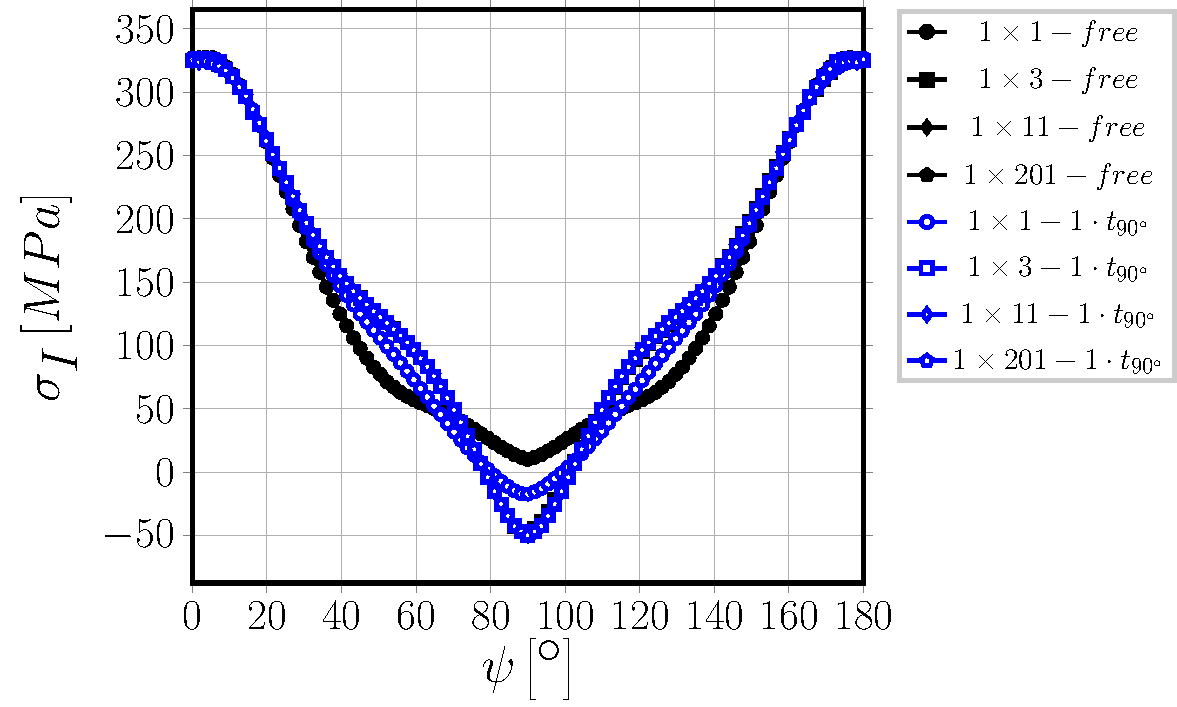
\includegraphics[height=0.22\textheight]{vf60-nodamage-sigmaI2D.pdf}}\ 
    \subfigure[$\sigma_{LMPS,3D}$]{\label{fig:stress-f}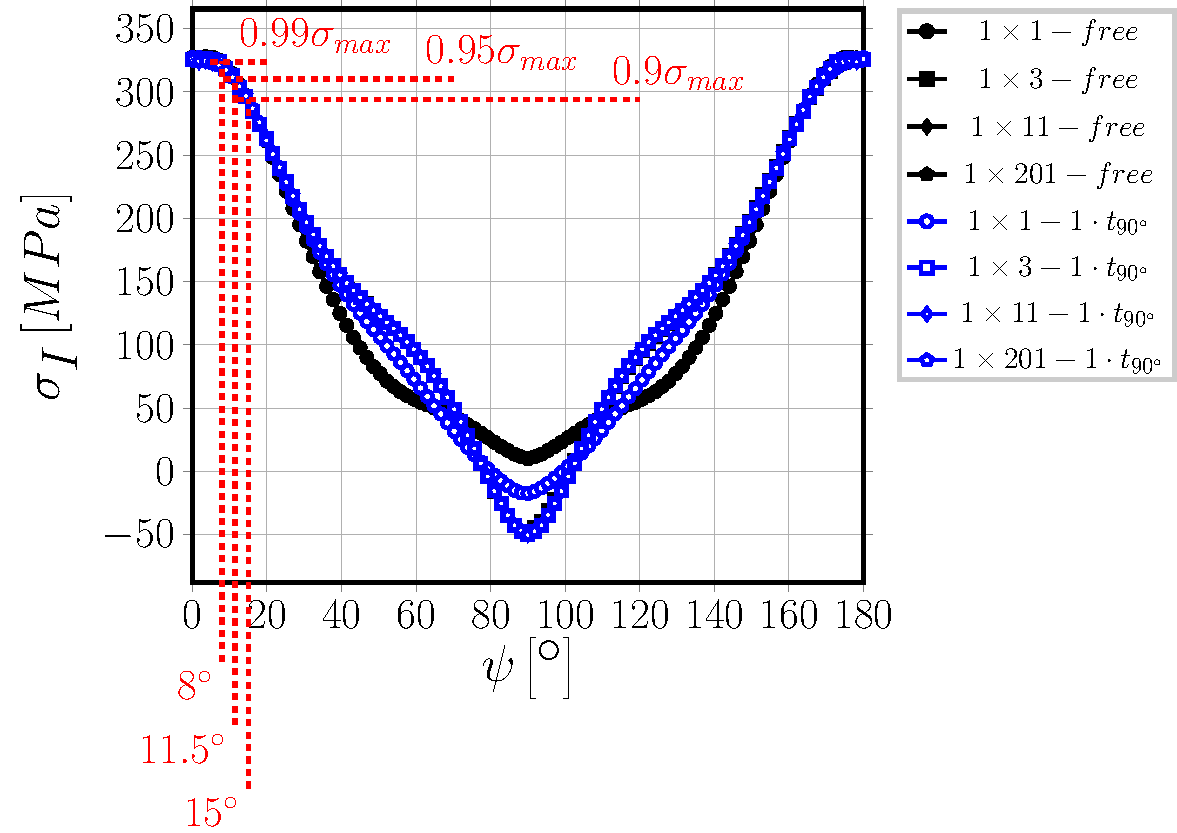
\includegraphics[height=0.22\textheight]{vf60-nodamage-sigmaI3D.pdf}}
\caption{Stress distribution at the fiber/matrix interface in the absence of damage.}\label{fig:stress}
\end{figure}

\section{ENERGY-BASED ANALYSIS OF DEBOND PROPAGATION}

\section{CONCLUSIONS}

We are looking forward to receiving your contributions for this conference.

\section*{ACKNOWLEDGEMENTS}

Luca Di Stasio gratefully acknowledges the support of the European School of Materials (EUSMAT) through the DocMASE Doctoral Programme and the European Commission through the Erasmus Mundus Programme.

\bibliographystyle{unsrt}

%\begin{thebibliography}{10}
%
%\bibitem{Barbero} E.J. Barbero, \textit{Finite Element Analysis of Composite Materials}. CRC Press, Boca Raton, 2008.
%\bibitem{Pimenta} S. Pimenta, S.T. Pinho, The effect of recycling on the mechanical response of carbon fibres and their composites. \textit{Composite Structures}, \textbf{94}, 3669-3684, 2012.
%
%\end{thebibliography}

\bibliography{refs}

\end{document}

